\documentclass[twoside]{book}

% Packages required by doxygen
\usepackage{fixltx2e}
\usepackage{calc}
\usepackage{doxygen}
\usepackage[export]{adjustbox} % also loads graphicx
\usepackage{graphicx}
\usepackage[utf8]{inputenc}
\usepackage{makeidx}
\usepackage{multicol}
\usepackage{multirow}
\PassOptionsToPackage{warn}{textcomp}
\usepackage{textcomp}
\usepackage[nointegrals]{wasysym}
\usepackage[table]{xcolor}

% Font selection
\usepackage[T1]{fontenc}
\usepackage[scaled=.90]{helvet}
\usepackage{courier}
\usepackage{amssymb}
\usepackage{sectsty}
\renewcommand{\familydefault}{\sfdefault}
\allsectionsfont{%
  \fontseries{bc}\selectfont%
  \color{darkgray}%
}
\renewcommand{\DoxyLabelFont}{%
  \fontseries{bc}\selectfont%
  \color{darkgray}%
}
\newcommand{\+}{\discretionary{\mbox{\scriptsize$\hookleftarrow$}}{}{}}

% Page & text layout
\usepackage{geometry}
\geometry{%
  a4paper,%
  top=2.5cm,%
  bottom=2.5cm,%
  left=2.5cm,%
  right=2.5cm%
}
\tolerance=750
\hfuzz=15pt
\hbadness=750
\setlength{\emergencystretch}{15pt}
\setlength{\parindent}{0cm}
\setlength{\parskip}{3ex plus 2ex minus 2ex}
\makeatletter
\renewcommand{\paragraph}{%
  \@startsection{paragraph}{4}{0ex}{-1.0ex}{1.0ex}{%
    \normalfont\normalsize\bfseries\SS@parafont%
  }%
}
\renewcommand{\subparagraph}{%
  \@startsection{subparagraph}{5}{0ex}{-1.0ex}{1.0ex}{%
    \normalfont\normalsize\bfseries\SS@subparafont%
  }%
}
\makeatother

% Headers & footers
\usepackage{fancyhdr}
\pagestyle{fancyplain}
\fancyhead[LE]{\fancyplain{}{\bfseries\thepage}}
\fancyhead[CE]{\fancyplain{}{}}
\fancyhead[RE]{\fancyplain{}{\bfseries\leftmark}}
\fancyhead[LO]{\fancyplain{}{\bfseries\rightmark}}
\fancyhead[CO]{\fancyplain{}{}}
\fancyhead[RO]{\fancyplain{}{\bfseries\thepage}}
\fancyfoot[LE]{\fancyplain{}{}}
\fancyfoot[CE]{\fancyplain{}{}}
\fancyfoot[RE]{\fancyplain{}{\bfseries\scriptsize Generated by Doxygen }}
\fancyfoot[LO]{\fancyplain{}{\bfseries\scriptsize Generated by Doxygen }}
\fancyfoot[CO]{\fancyplain{}{}}
\fancyfoot[RO]{\fancyplain{}{}}
\renewcommand{\footrulewidth}{0.4pt}
\renewcommand{\chaptermark}[1]{%
  \markboth{#1}{}%
}
\renewcommand{\sectionmark}[1]{%
  \markright{\thesection\ #1}%
}

% Indices & bibliography
\usepackage{natbib}
\usepackage[titles]{tocloft}
\setcounter{tocdepth}{3}
\setcounter{secnumdepth}{5}
\makeindex

% Hyperlinks (required, but should be loaded last)
\usepackage{ifpdf}
\ifpdf
  \usepackage[pdftex,pagebackref=true]{hyperref}
\else
  \usepackage[ps2pdf,pagebackref=true]{hyperref}
\fi
\hypersetup{%
  colorlinks=true,%
  linkcolor=blue,%
  citecolor=blue,%
  unicode%
}

% Custom commands
\newcommand{\clearemptydoublepage}{%
  \newpage{\pagestyle{empty}\cleardoublepage}%
}

\usepackage{caption}
\captionsetup{labelsep=space,justification=centering,font={bf},singlelinecheck=off,skip=4pt,position=top}

%===== C O N T E N T S =====

\begin{document}

% Titlepage & ToC
\hypersetup{pageanchor=false,
             bookmarksnumbered=true,
             pdfencoding=unicode
            }
\pagenumbering{alph}
\begin{titlepage}
\vspace*{7cm}
\begin{center}%
{\Large Test comments }\\
\vspace*{1cm}
{\large Generated by Doxygen 1.8.13}\\
\end{center}
\end{titlepage}
\clearemptydoublepage
\pagenumbering{roman}
\tableofcontents
\clearemptydoublepage
\pagenumbering{arabic}
\hypersetup{pageanchor=true}

%--- Begin generated contents ---
\chapter{Hierarchical Index}
\section{Class Hierarchy}
This inheritance list is sorted roughly, but not completely, alphabetically\+:\begin{DoxyCompactList}
\item App\+Compat\+Activity\begin{DoxyCompactList}
\item \contentsline{section}{com.\+example.\+alex.\+victorreader.\+Main\+Activity}{\pageref{classcom_1_1example_1_1alex_1_1victorreader_1_1_main_activity}}{}
\end{DoxyCompactList}
\end{DoxyCompactList}

\chapter{Class Index}
\section{Class List}
Here are the classes, structs, unions and interfaces with brief descriptions\+:\begin{DoxyCompactList}
\item\contentsline{section}{\hyperlink{classcom_1_1example_1_1alex_1_1victorreader_1_1_main_activity}{com.\+example.\+alex.\+victorreader.\+Main\+Activity} }{\pageref{classcom_1_1example_1_1alex_1_1victorreader_1_1_main_activity}}{}
\end{DoxyCompactList}

\chapter{Class Documentation}
\hypertarget{classcom_1_1example_1_1alex_1_1victorreader_1_1_main_activity}{}\section{com.\+example.\+alex.\+victorreader.\+Main\+Activity Class Reference}
\label{classcom_1_1example_1_1alex_1_1victorreader_1_1_main_activity}\index{com.\+example.\+alex.\+victorreader.\+Main\+Activity@{com.\+example.\+alex.\+victorreader.\+Main\+Activity}}
Inheritance diagram for com.\+example.\+alex.\+victorreader.\+Main\+Activity\+:\begin{figure}[H]
\begin{center}
\leavevmode
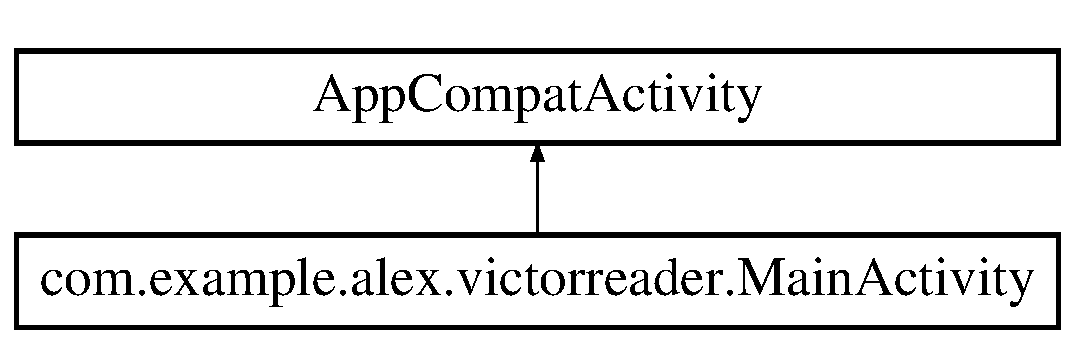
\includegraphics[height=2.000000cm]{classcom_1_1example_1_1alex_1_1victorreader_1_1_main_activity}
\end{center}
\end{figure}
\subsection*{Public Attributes}
\begin{DoxyCompactItemize}
\item 
Text\+To\+Speech \hyperlink{classcom_1_1example_1_1alex_1_1victorreader_1_1_main_activity_a0ed6c05d6b216e7c01692c11ff660578}{tts}
\end{DoxyCompactItemize}
\subsection*{Protected Member Functions}
\begin{DoxyCompactItemize}
\item 
void \hyperlink{classcom_1_1example_1_1alex_1_1victorreader_1_1_main_activity_ad3ee93762ef61943471e7253eaa9a7be}{on\+Create} (Bundle saved\+Instance\+State)
\end{DoxyCompactItemize}


\subsection{Member Function Documentation}
\mbox{\Hypertarget{classcom_1_1example_1_1alex_1_1victorreader_1_1_main_activity_ad3ee93762ef61943471e7253eaa9a7be}\label{classcom_1_1example_1_1alex_1_1victorreader_1_1_main_activity_ad3ee93762ef61943471e7253eaa9a7be}} 
\index{com\+::example\+::alex\+::victorreader\+::\+Main\+Activity@{com\+::example\+::alex\+::victorreader\+::\+Main\+Activity}!on\+Create@{on\+Create}}
\index{on\+Create@{on\+Create}!com\+::example\+::alex\+::victorreader\+::\+Main\+Activity@{com\+::example\+::alex\+::victorreader\+::\+Main\+Activity}}
\subsubsection{\texorpdfstring{on\+Create()}{onCreate()}}
{\footnotesize\ttfamily void com.\+example.\+alex.\+victorreader.\+Main\+Activity.\+on\+Create (\begin{DoxyParamCaption}\item[{Bundle}]{saved\+Instance\+State }\end{DoxyParamCaption})\hspace{0.3cm}{\ttfamily [protected]}}

Method that controls what happens when the record button is clicked It creates a Media\+Recorder object to be used and sets up the destination path for the file. It uses the date and time for filename and starts recording until the stop button is clicked.

Method that controls what happens when the stop button is clicked This button only appears after the record button has been clicked. It releases the Media\+Recorder object used and updates the list of audio files to include the audio that was just recorded.

Method that controls what happens when the play\+Back button is clicked This is responsible for playing back the audio files recorded. It uses the file selected from the navigate button.

Method that controls what happens when the navigate button is clicked It cycles through the list of files and reads the filename aloud that could be played back.

\subsection{Member Data Documentation}
\mbox{\Hypertarget{classcom_1_1example_1_1alex_1_1victorreader_1_1_main_activity_a0ed6c05d6b216e7c01692c11ff660578}\label{classcom_1_1example_1_1alex_1_1victorreader_1_1_main_activity_a0ed6c05d6b216e7c01692c11ff660578}} 
\index{com\+::example\+::alex\+::victorreader\+::\+Main\+Activity@{com\+::example\+::alex\+::victorreader\+::\+Main\+Activity}!tts@{tts}}
\index{tts@{tts}!com\+::example\+::alex\+::victorreader\+::\+Main\+Activity@{com\+::example\+::alex\+::victorreader\+::\+Main\+Activity}}
\subsubsection{\texorpdfstring{tts}{tts}}
{\footnotesize\ttfamily Text\+To\+Speech com.\+example.\+alex.\+victorreader.\+Main\+Activity.\+tts}

Texttoooospech var very goo description 

The documentation for this class was generated from the following file\+:\begin{DoxyCompactItemize}
\item 
Main\+Activity.\+java\end{DoxyCompactItemize}

%--- End generated contents ---

% Index
\backmatter
\newpage
\phantomsection
\clearemptydoublepage
\addcontentsline{toc}{chapter}{Index}
\printindex

\end{document}
